\documentclass[a4paper, 12pt]{article}%тип документа

%%%Библиотеки
	%\usepackage[warn]{mathtext}	
	\usepackage[T2A]{fontenc} % кодировка
	\usepackage[utf8]{inputenc} % кодировка исходного текста
	\usepackage[english,russian]{babel} % локализация и переносы
	\usepackage{caption}
	\usepackage{listings}
	\usepackage{amsmath,amsfonts,amssymb,amsthm,mathtools}
	\usepackage{wasysym}
	\usepackage{graphicx}%Вставка картинок правильная
	\usepackage{float}%"Плавающие" картинки
	\usepackage{wrapfig}%Обтекание фигур (таблиц, картинок и прочего)
	\usepackage{fancyhdr} %загрузим пакет
	\usepackage{lscape}
	\usepackage{xcolor}
	\usepackage[normalem]{ulem}
	\usepackage{hyperref}

%%%Конец библиотек




%%%Настройка ссылок
	\hypersetup
	{
		colorlinks=true,
		linkcolor=blue,
		filecolor=magenta,
		urlcolor=blue
	}
%%%Конец настройки ссылок


%%%Настройка колонтитулы
	\pagestyle{fancy}
	\fancyhead{}
	\fancyhead[L]{Лабораторная работа}
	\fancyhead[R]{Талашкевич Даниил, группа Б01-008}
	\fancyfoot[C]{\thepage}
%%%конец настройки колонтитулы



							\begin{document}
						%%%%Начало документа%%%%


%%%Начало титульника
\begin{titlepage}

	\newpage
	\begin{center}
		\normalsize Московский физико-технический институт \\(госудраственный 			университет)
	\end{center}

	\vspace{6em}

	\begin{center}
		\Large Лабораторная работа по квантовой физике\\
	\end{center}

	\vspace{1em}

	\begin{center}
		\large \textbf{Изучение рассеяния медленных электронов на атомах (эффект Рамзауэра) [1.3]}
	\end{center}

	\vspace{2em}

	\begin{center}
		\large Талашкевич Даниил Александрович\\
		Группа Б01-008
	\end{center}

	\vspace{\fill}

	\begin{center}
	Долгопрудный \\2022
	\end{center}
	
\end{titlepage}
%%%Конец Титульника



%%%Настройка оглавления и нумерации страниц
	\thispagestyle{empty}
	\newpage
	\tableofcontents
	\newpage
	\setcounter{page}{1}
%%%Настройка оглавления и нумерации страниц


					%%%%%%Начало работы с текстом%%%%%%

\section{Аннотация}

\ \ \ \textbf{Цель работы:} исследовать энергетическую зависимость вероятности рассеяния электронов атомами инертного газа, определить энергию электронов при которых наблюдается <<просветление>> инертного газа и оценить размер его внешней электронной оболочки.

\textbf{Оборудование}: тиратрон ТГ3-01/1.3Б, эскпериментальная блок-схема, осциллограф, вольтметры, амперметры.

\subsection{Теория}
Рассеяние электрона на атоме можно приближённого рассматривать как рассеяние частицы энергии $E$ на потенциальной яме длины $\ell$ и глубины $U_0$. Уравнение Шрёдингера имеет вид
\[\Psi'' + k^2 \Psi = 0,\]
где вне ямы 
\[k^2 = k_1^2 = \dfrac{2mE}{\hbar^2},\]
а внутри 
\[k^2 = k_2^2 = \dfrac{2m(E+U_0)}{\hbar^2}.\]
Коэффициент прохождения в таком случае равен
\[D = \dfrac{16 k_1^2 k_2^2}{16k_1^2 k_2^2 + 4(k_1^2 - k_2^2)^2\sin^2(k_2\ell)}.\]
Заметим, что коэффициент прохождения имеет ряд максимумов и минимумов. Он максимальнем при
\begin{equation}\label{0}
\sqrt{\dfrac{2m(E+U_0)}{\hbar^2}}\ell = n\pi,~n=1,2,3,\dots
\end{equation}

Качественно эффект Рамзауэра можно объяснить, рассмотрев интерференцию прошедшей и дважды отразившейся от оболочки волн де Бройля. Длины волн вне и внутри атома:
\[\lambda = \dfrac{h}{\sqrt{2mE}},~\lambda_1 = \dfrac{h}{\sqrt{2m(E+U_0)}}.\]
Соответственно условия на первые интерфереционные максимум и минимум 
\begin{equation}\label{1}
2\ell = \dfrac{h}{\sqrt{2m(E_1 + U_0)}},~2\ell = \dfrac{3}{2}\dfrac{h}{\sqrt{2m(E_2 + U_0)}},
\end{equation}

где $E_1, E_2$ - энергии, соответствующие максимуму и минимуму прохождения электронов соответственно.


Исключая из этих соотношений глубину ямы, получим
\begin{equation}\label{2}
\ell = \dfrac{h\sqrt{5}}{\sqrt{32m(E_2 - E_1)}}.
\end{equation}
Глубина ямы при этом равна
\begin{equation}\label{4}
U_0 = \dfrac{4}{5}E_2 - \dfrac{9}{5}E_1.
\end{equation}
\subsection{Описание установки}

\begin{figure}[h]
    \center{{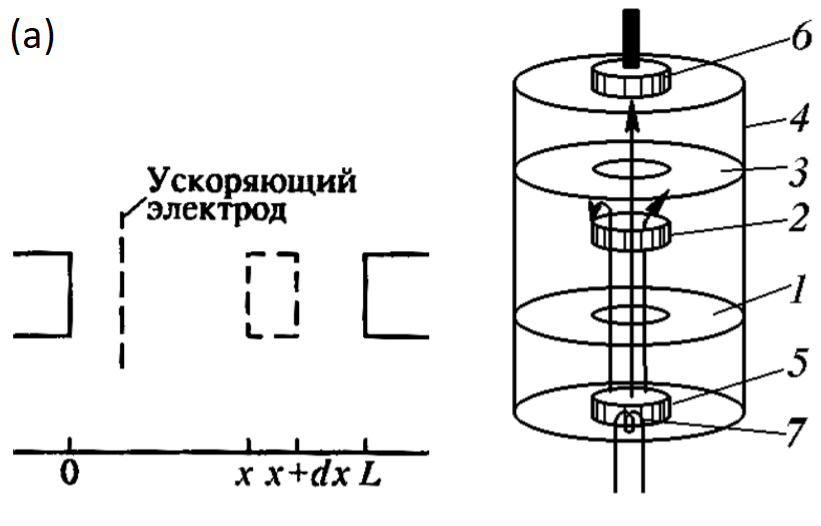
\includegraphics[width=0.42\textwidth]{img/2.png}}}
    \center{{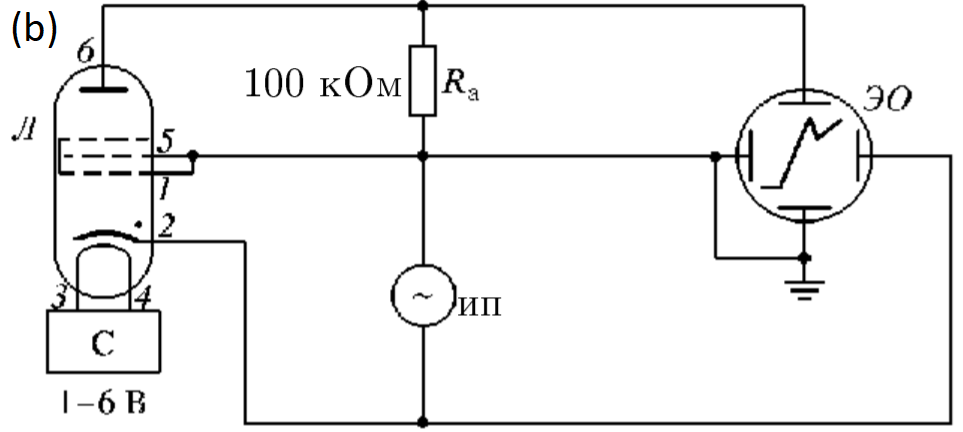
\includegraphics[width=0.58\textwidth]{img/3.png}}}
  \centering
  \caption{(a) Схема тиратрона (слева) и его конструкция (справа): 1,2,3 -- сетки, 4 -- внешний металлический цилиндр, 5 -- катод, 6 -- анод, 7 -- накаливаемая спираль. (b) Схема включения тиратрона.}
\end{figure}
Для изучения эффекта испульзуется тиратрон ТГ3-01/1.3Б, заполненный инертным газом (Рис. 1а). Электроны эмитируются катодом, ускоряются напряжением $V$ и рассеиваются на атомах газа. Сетки соединены между собой и имеют один потенциал, примерно равный потенциалу анода. Рассеянные электроны отклоняются и уходят на сетку, а оставшиеся достигают анода, создавая ток $I_\text{a}$. Таким образом, поток электронов на расстоянии $x$ от ускоряющей сетки уменьшается с ростом $x$. ВАХ анода должна быть
\begin{equation}\label{3}
I_\text{a} = I_0 \exp\left( - C w(V) \right),
\end{equation}
где $I_0 = eN_0$ -- ток катода, $I_\text{a} = eN_a$ -- ток анода, $C = Ln_\text{a} \Delta_\text{a}$($L$ --  расстояние между катодом и анодом, $\Delta_\text{a}$ -- площадь поперечного сечения атома, $n_\text{a}$ -- концентрация газа в лампе), $w(V)$ -- вероятность рассеяния на атоме.
Формулу \eqref{3} можно переписать в виде
\[\tag{5a}\label{5a}
w(V) = -\dfrac{1}{C}\ln \dfrac{I_\text{a}(V)}{I_0}.
\]
\begin{figure}[h]
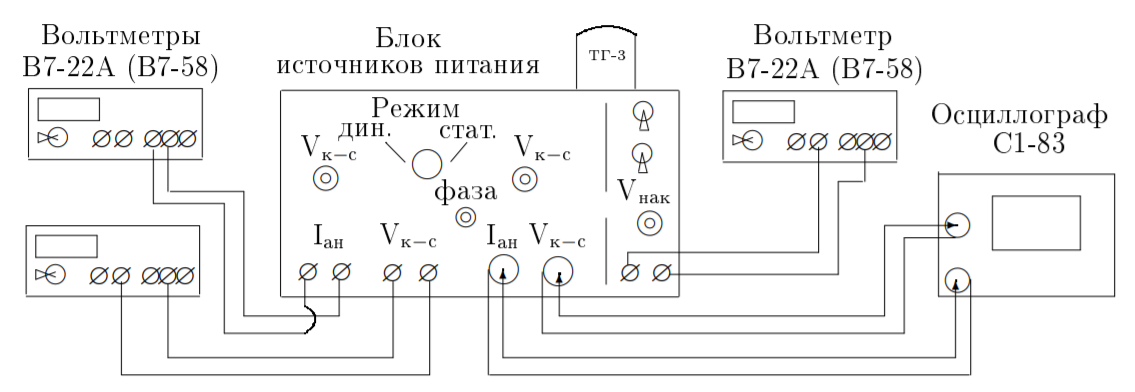
\includegraphics[scale=0.6]{img/1.png}
\centering
\caption{Схема установки.}
\end{figure}\\
Схема экспериментальной установки, изображанная на Рис. 1b, в нашей работе конструктивно осуществлена следующим образом (Рис. 2): лампа-тиратрон расположена непосредственно на корпусе блока источников питания (БИП), напряжение к электродам лампы подаётся от источников питания, находящихся в корпусе прибора. Регулировка напряжения и выбор режима работы установки производится при помощи ручек управления, выведенных на лицевую панель БИП.

\newpage

\section{Ход работы}

\subsection{Данные}



\begin{table}[!h] 
		\begin{tabular}{|c|c|c|c|c|c|c|c|c|c|c|}
\hline & \multicolumn{10}{|c|}{$U_{\text {накала }}=2.61 \mathrm{~B}$}\\
\hline$U, \mathrm{~B}$ & $2.639$ & $3.162$ & $3.566$ & $4.111$ & $4.502$ & $5.299$ & $4.737$ & $6.325$ & $6.802$ & $7.095$\\
$I_{\mathrm{a}}, \mathrm{мA}$ & $0.0295$ & $0.18$ & $0.216$ & $0.227$ & $0.228$ & $0.212$ & $0.229$ & $0.187$ & $0.172$ & $0.162$ \\
\hline$U, \mathrm{~B}$ & $8.232$ & $9.488$ & $10.625$ & $11.006$ & $11.588$ & $11.528$ & $12.197$ & $12.193$ & $7.503$  &  \\
$I_{\mathrm{a}}, \mathrm{mA}$ & $0.126$ & $0.103$ & $0.099$ & $0.1012$ & $0.106$ & $0.105$ & $0.110$ & $0.110$ & $0.147$ & \\
\hline
	\end{tabular}
\end{table}

\begin{table}[!h]
		\begin{tabular}{|c|c|c|c|c|c|c|c|c|c|c|c|}
\hline & \multicolumn{10}{|c|}{$U_{\text {накала }}=2.97 \mathrm{~B}$} &\\
\hline$U, \mathrm{~B}$ & $2.979$ & $3.261$ & $3.514$ & $3.858$ & $4.045$ & $4.435$ & $5.028$ & $5.252$ & $5.424$ & $6.032$ & $6.248$ \\
$I_{\mathrm{a}}, \mathrm{мA}$ & $0.383$ & $0.474$ & $0.537$ & $0.600$ & $0.629$ & $0.675$ & $0.709$ & $0.715$ & $0.717$ & $0.712$ & $0.707$ \\

\hline$U, \mathrm{~B}$ & $6.557$ & $6.730$ & $7.047$ & $7.472$ & $7.856$ & $8.712$ & $9.515$ & $10.394$ & $10.701$ & $ 11.28$ & $10.713$\\
$I_{\mathrm{a}}, \mathrm{mA}$ & $0.693$ & $0.683$ & $0.659$ & $0.621$ & $0.586$ & $0.518$ & $0.468$ & $0.459$ & $0.465$ & $0.484$ & $0.469$\\
\hline
	\end{tabular}
\caption{Результаты измерений в статическом режиме}
\end{table} 

\begin{table}[!h] \begin{center}
	\begin{tabular}{|c|c|c|c|c|}
		\hline$V_{\text{накала}}, \mathrm{~B}$ & $V_{min},\ B$ & $V_{\text{max}},\ B$ & $V_{\text {пробоя}}, \text{В}$ & $\text{расст. до мин, В}$\\
		\hline 2,97 & 8,2 & 3,2 & 16,4 & 10,0 \\
		\hline 2,61 & 7,0 & 3,0 & 17,2  & 5,8 \\
		\hline
	\end{tabular}
\caption{Результаты измерений в динамическом режиме}
\end{center} \end{table}	

%\newpage

%\begin{table}[!h] \begin{center}
%	\begin{tabular}{|c|c|c|c|}
%		\hline & $V, \mathrm{~B}$ & $U$, В & $I$, мA 		\\
%		\hline Величина & 2,65 & 5,0 & 1,00 \\
%		\hline Погрешность & 0,02 & 0,1 & 0,05 \\
%		\hline$\varepsilon, \%$ & 1,0 & 2,0 & 5,0 \\
%		\hline
%	\end{tabular}
%\caption{Некоторые измеряемые величины и их погрешность.}
%\end{center} \end{table}


\newpage	

\subsection{Обработка данных}

\begin{enumerate}

\item Используя формулы $\ref{1}$ рассчитаем размер электронной оболочки атома инертного газа ($V_{min} = 8.2 B,\ V_{max} = 3.2 B,\ V_0 = 1,28 B$):

\begin{equation*}
2\ell = \dfrac{h}{\sqrt{2m(E_1 + U_0)}} = 580 \pm 55 \text{пм},~2\ell = \dfrac{3}{2}\dfrac{h}{\sqrt{2m(E_2 + U_0)}} = 598 \pm 58 \text{пм},
\end{equation*}

Теперь рассчитаем по формуле $\ref{2}:$

\begin{equation*}
\ell = \dfrac{h\sqrt{5}}{\sqrt{32m(E_2 - E_1)}} = 388 \pm 35 \text{пм}.
\end{equation*}

\item Оценим глубину потенциальной ямы по формуле $\ref{4}:$

\begin{equation*}
U_0 = \dfrac{4}{5}E_2 - \dfrac{9}{5}E_1 = 1.28 \pm 0.29\text{эB}.
\end{equation*}

\item По результатам измерений напряжения пробоя оценим потенциал ионизации инертного газа:

Получили что тиратрон наполнен аргоном.

\item Построем графики $I_{\mathrm{a}}=f\left(V_{\mathrm{c}}\right)$ (для статического режима):


\begin{figure}[!h]
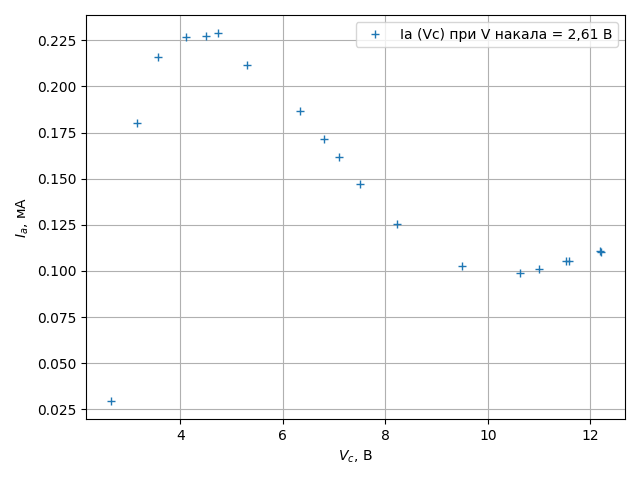
\includegraphics[scale=0.6]{I_V_static_261.png}
\centering
\caption{$V_{\text{накала}}$ = 2.61 В}
\label{graph1}
\end{figure}

\begin{figure}[!h]
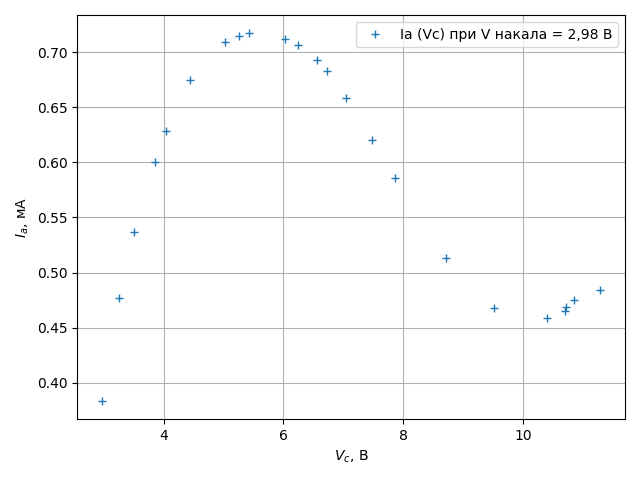
\includegraphics[scale=0.6]{I_V_static_298.png}
\centering
\caption{$V_{\text{накала}}$ = 2.98 В}
\label{graph2}
\end{figure}

%\begin{figure}[!h]
%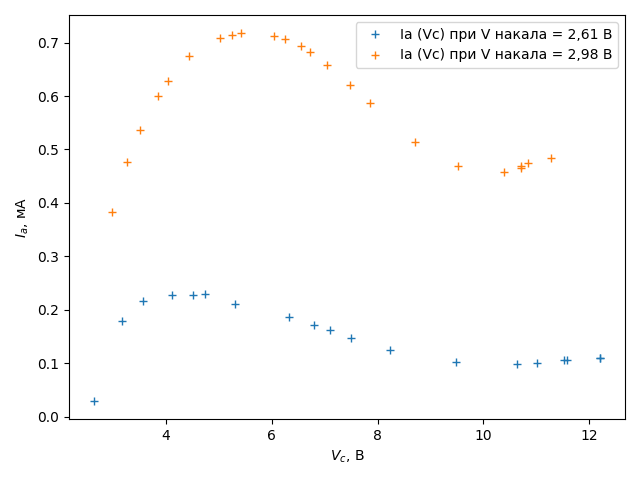
\includegraphics[scale=0.6]{I_V_static_both.png}
%\centering
%\caption{оба}
%\label{graph_both}
%\end{figure}

\item Оценим, используя ф-лу:

$$
k_2 l=\sqrt{\frac{2 m\left(E_n+U_0\right)}{\hbar^2}} l=n \pi, \quad n=1,2,3,
$$

определим, при каких напряжениях должны появляться максимумы в коэффициенте прохождения электронов для $n=2,3$. Сравним полученные величины с наблюдаемыми особенностями на BAX тиратрона.

\item На основе формулы $\ref{5a}$ найдем зависимость вероятности рассеяния элект ронов (с точно стью до константы) от энергии и построим соответствующие графики:

\newpage

\begin{figure}[!h]
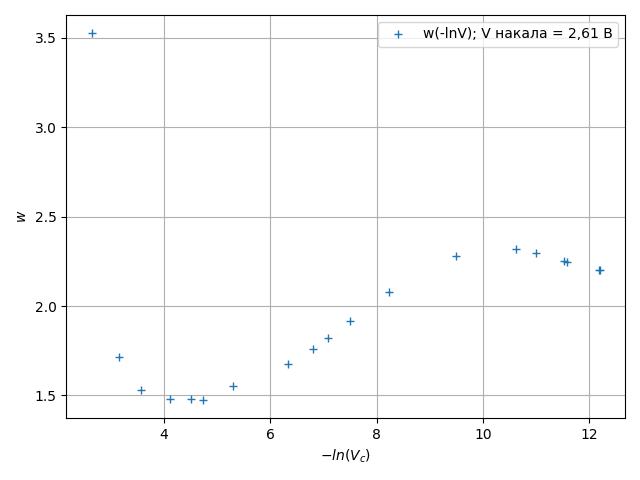
\includegraphics[scale=0.6]{w_v_61.png}
\centering
\caption{$V_{\text{накала}}$ = 2.61 В}
\label{graph3}
\end{figure}

\begin{figure}[!h]
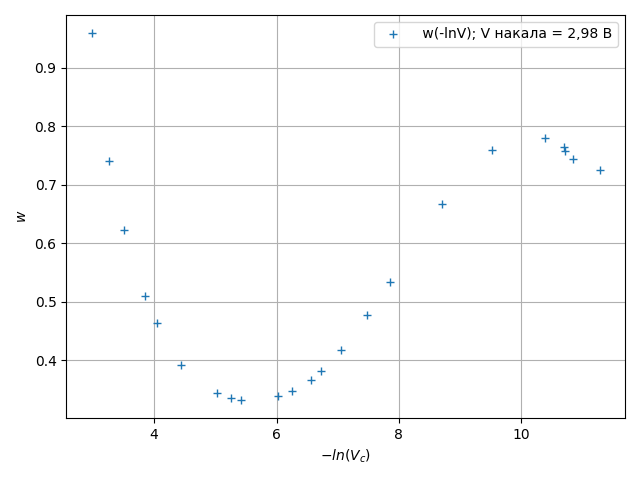
\includegraphics[scale=0.6]{w_v_98.png}
\centering
\caption{$V_{\text{накала}}$ = 2.98 В}
\label{graph4}
\end{figure}

Из линейного участка графика по МНК найдем $k$ -- коэф. наклона, $\text{где } k = \frac{1}{C}$:

$$ k_1 = 0.105 \pm 0.012;\ k_2 = 0.090 \pm 0.007$$
$$ C_1 = 9.52 \pm 1,088;\ C_2 = 11.11 \pm 0.864;\ \Delta C = \frac{1}{k^2}\cdot \Delta k$$

\item ВАХ тиратрона в динамическом режиме:

\begin{figure}[!h]
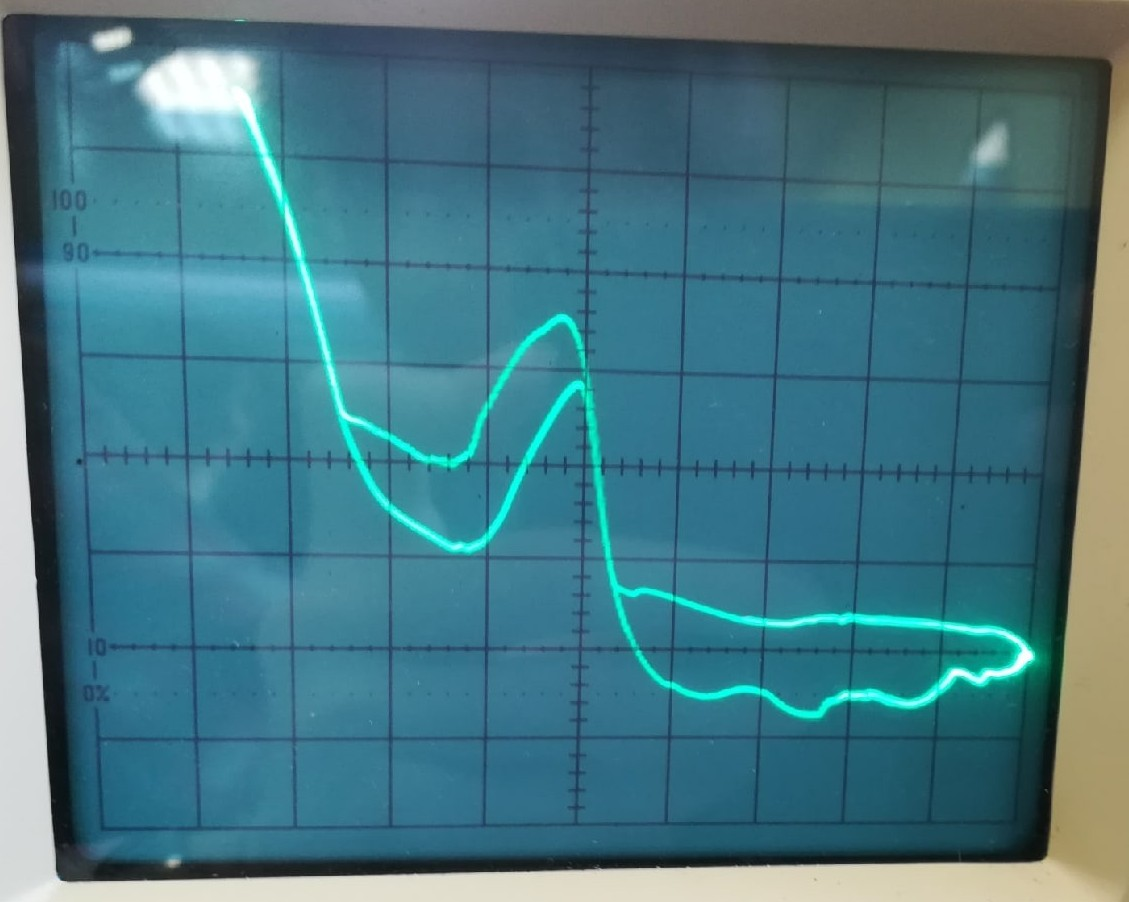
\includegraphics[scale=0.25]{dynam_61.jpg}
\centering
\caption{$V_{\text{накала}}$ = 2.61 В}
\label{graph5}
\end{figure}

\begin{figure}[!h]
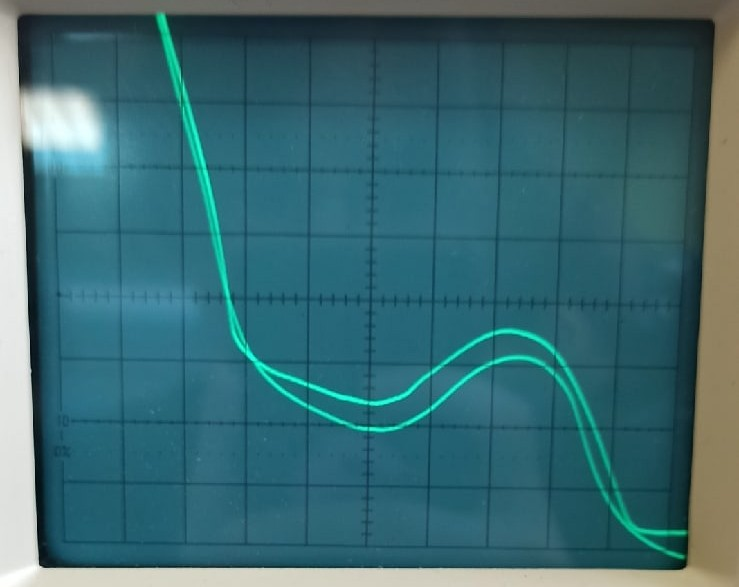
\includegraphics[scale=0.4]{dynam_97.jpg}
\centering
\caption{$V_{\text{накала}}$ = 2.97 В}
\label{graph6}
\end{figure}


\item Погрешности оценим по формулам:
		\begin{equation*}
			\sigma_{l_1} = l_1 \frac{\sigma_{E_1}}{E_1}, \ \sigma_{l_2} = l_2 \frac{\sigma_{E_2}}{E_2}, \ \sigma_{l_3} = l_3 \frac{\sigma_{E_1}+\sigma_{E_2}}{E_2-E_1}.
		\end{equation*}

	Погрешность определения константы $C$ в $\ref{5a}$ находилась из МНК.

\end{enumerate}


\newpage

\section{Вывод}

В ходе лабораторной работы мы наблюдали ВАХ тиратрона в динамическом режиме (рис.$~\ref{graph1},~\ref{graph6}$) при различных напряжениях накала, причем по напряжению пробоя определили, что используемый в эксперименте инертный газ состоит из атомов ксенона. Действительно, энергия ионизации ксенона -- 16,4 эв, а $E_\text{пробоя} = (16,2 \pm 0,5)$ эВ. 
	
	Вольт-амперная характеристика тиратрона в статическом режиме \\
(рис. $\ref{graph1},~\ref{graph2}$) имеет вид, который находится в согласии с квантовой теорией. Электрон, обладая волновыми свойствами, способен <<интерферировать сам с собой>> при рассеянии на атоме, тем самым усиливая или ослабевая анодный ток. Энергии электрона (напряжения на катоде) при которых наблюдаются максимумы или минимумы в статическом режиме примерно совпадают со значениями, полученными при измерениях в динамическом режиме.
	
	Проанализируем вид зависимости $w = w(U)$, представленной на рис. ($\ref{graph3},~\ref{graph4}$) , при напряжении накала $V = 2,62$ В с точностью до константы $C$. На графике в диапазоне от 1В до 12В отчетливо видны максимум и минимум, что подтверждает справдливость эффекта Рамзауэра -- эффективное сечение реакции сильно зависит от энергии электрона. Однако видно, что при достаточно малых энергиях электрона погрешность вероятности сильно возрастает, что неудивительно, ведь из формулы ($\ref{5a}$) видно, что $w\rightarrow +\infty$ при $U\rightarrow0$ (этот предел не зависит от нормировачной константы $C$), что противоречит физической реальности. Можно сделать вывод, что формула ($\ref{5a}$) имеет границы применимости: энергия электрона $E \geq 1$ эВ. При меньших энергиях электрон может испытывать другие квантовые эффекты: рассеяние медленных частиц, резонансное рассеяние при малых энергиях.



\section{Литература}

\begin{enumerate}

\item Лабораторный практикум по общей физике. Квантовая физика.

\item МНК -- http://mathhelpplanet.com/static.php?p=onlayn-mnk-i-regressionniy-analiz

\end{enumerate}	

\end{document}
